\section{Data and methods}
\subsection{General workflow}
\justify
This chapter describes the usage of methods in this study.

\begin{itemize}
    \item Kyselytutkimuksen teko
    \item Kyselytutkimuksen toteuttaminen
    \item geoprosessointi ja visualisointien tuotto
    \item Kyselytutkimuksen tulostentutkimus
    \item lopussa upea flowchartti
\end{itemize}

\begin{figure}[H]
    \centering
    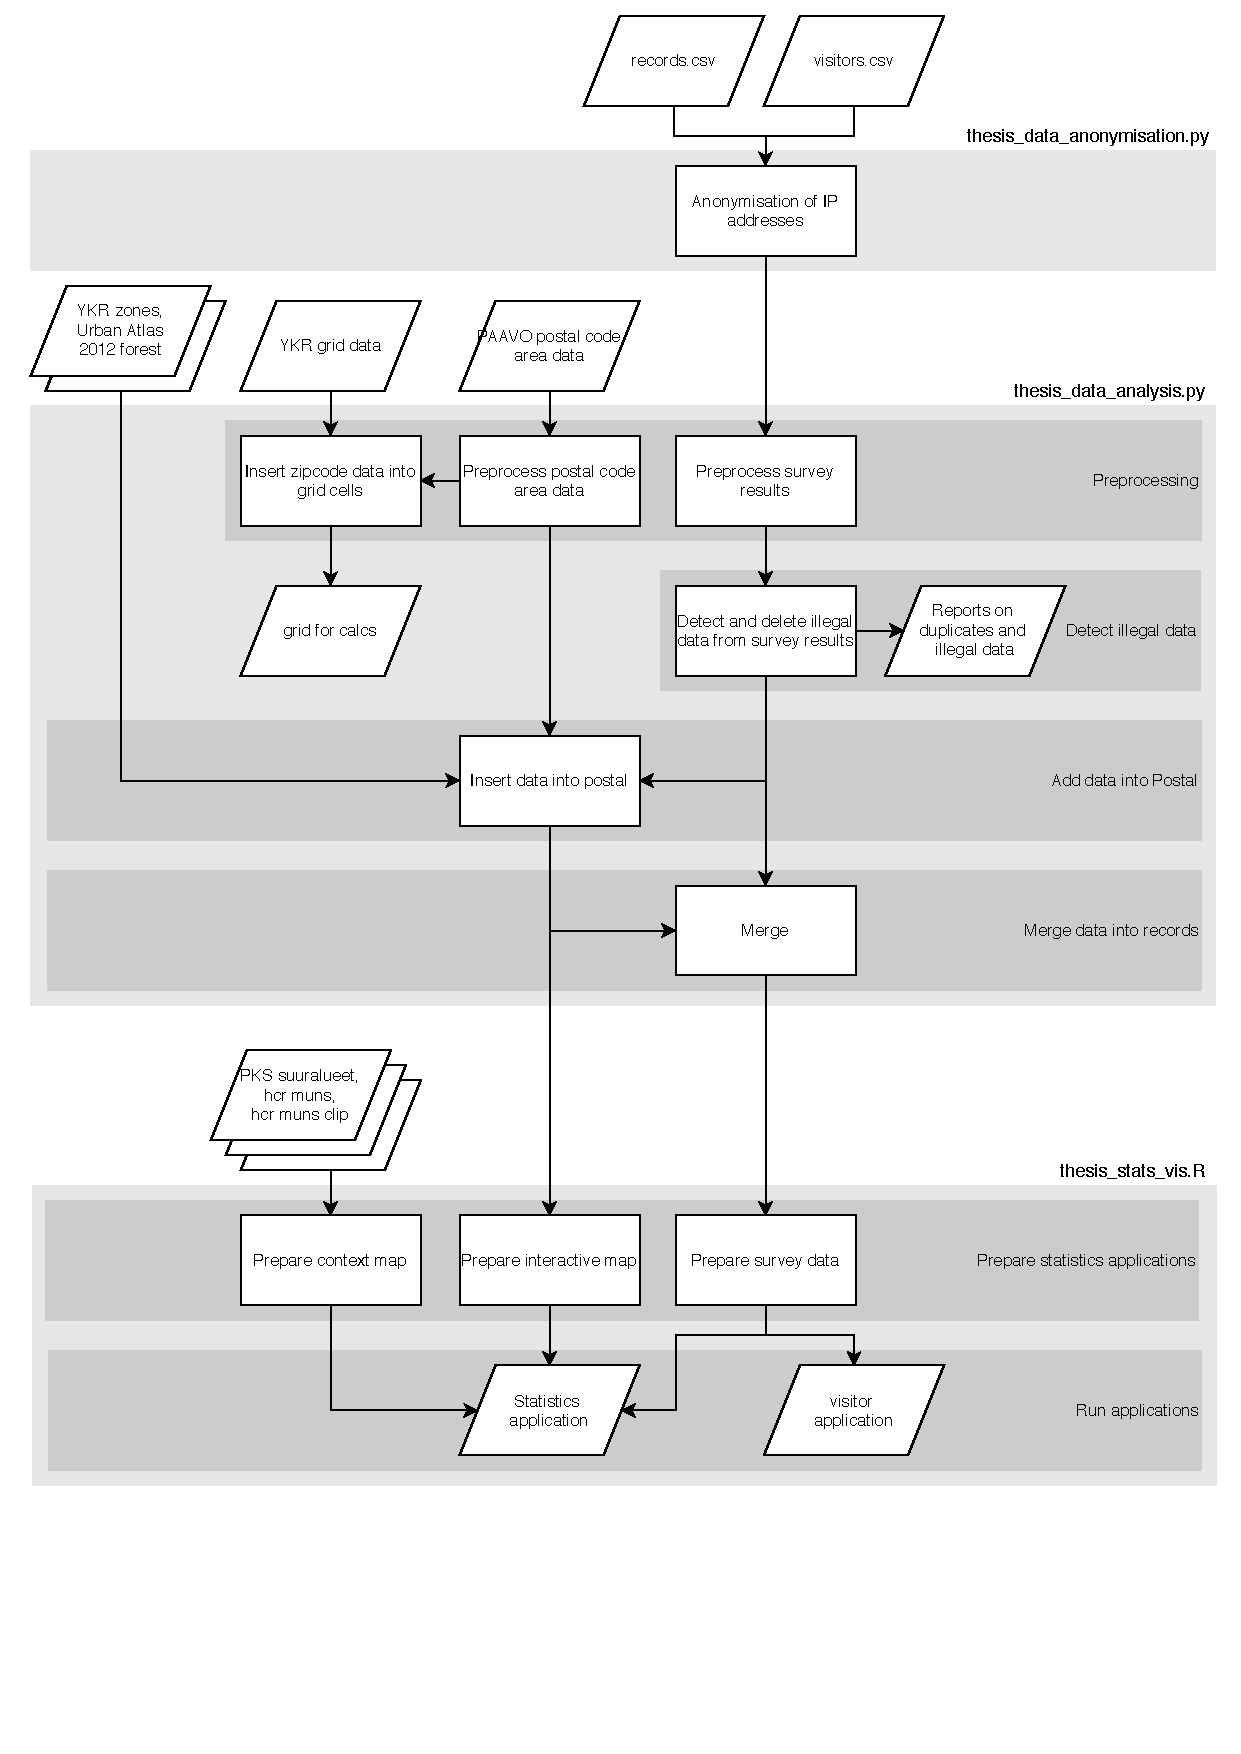
\includegraphics[trim=0.5cm 4.5cm 0.5cm 0.5cm,width=\columnwidth,scale=0.5]{thesis_workflow.pdf}
    \caption{General workflow in Python and R.} 
    \label{fig:gen_workflow}
\end{figure}

\subsection{Study area}
\justify
% https://www.hel.fi/hel2/Helsinginseutu/HS_tunnusluvut/liikennemaara_ja_autonomistus.pdf
% https://www.hsl.fi/sites/default/files/19_2016_auton_omistus_helsingin_seudulla.pdf
% https://www.hsl.fi/tutkimukset/muut-selvitykset
% http://pxnet2.stat.fi/PXWeb/pxweb/fi/StatFin/StatFin__lii__mkan/
The study area of this thesis is the Helsinki Capital Region. It comprises of municipalities of Helsinki, Espoo, Vantaa and Kauniainen. According to \textcolor{red}{LÄHDE}, the total population of the metropolitan area is 1.495 million. In practice the whole area amalgamates as one complete functional area with borders of the municipalities indistinguishable at the street level. The Helsinki Capital Region faces increasing pressure to manage its traffic because \textcolor{red}{LÄHDE}. Of these four municipalities Helsinki is the hub, and considered to contain the only inner city features of the municipalities (\textcolor{red}{syke-urbanareas}). Espoo, Vantaa and Kauniainen mostly consists of suburban areas with occasional industrial areas and large shopping complexes placed throughout the area. The Helsinki Capital Region is served with a high performance public transport system comprised of buses, train, subway, and tram in Helsinki. Recently, in 2017, the subway expanded from Helsinki to Espoo, triggering a new phase of quickly evolving cityscape in the surroundings of the new stations.

(\textcolor{red}{Insert map of the research area})

Despite the extensive service level of Helsinki Capital Region public transport, households especially in Espoo, Vantaa, and Kauniainen remain dependent on their personal vehicles (\textcolor{red}{LÄHDE}). 

\subsection{Data}
\justify

% hyphenrules: prevent hyphenation temporarily
\begin{hyphenrules}{nohyphenation}
    \begin{table}[H]
        \centering
        \setlength\tabcolsep{1pt}
        \caption{Used data} 
        \label{tab:useddata}
        % One unit here is ">{\raggedright\arraybackslash}p{4cm}". \raggedright prevents justification of text and conveniently allows flush right or flush left, which is not possible with column command p{4cm} alone.
        \begin{tabular}{ @{} >{\raggedright\arraybackslash}p{4cm} >{\raggedright\arraybackslash}p{4cm} >{\raggedright\arraybackslash}p{4cm} >{\raggedleft\arraybackslash}p{2cm} @{} }
            \toprule
            \cmidrule(r){1-2}
            Data & Description & Producer & Citation \\
            \midrule
            Paavo -- Open data by postal code area & Postal code areas & Statistics Finland & 2 \\
            Urban Atlas 2012 & Land use and land cover data & European Environment Agency & \cite{EuropeanEnvironmentAgency2016Urban2012} \\
            Urban regions (Yhdyskuntarakenteen vyöhykkeet) 2017 & Zones of urban regions & Finnish Environment Institute & 1 \\
            Helsinki Region-Travel Time Matrix 2018 & Travel time and distance information for routes between all YKR grid cell centroids in the Capital Region of Helsinki & Digital Geography Lab & \cite{Tenkanen2018Helsinki2018} \\
            YKR grid & Statistical grid for 250 x 250 meters & Statistics Finland & 2 \\
            \bottomrule
        \end{tabular}
    \end{table} 
\end{hyphenrules}

\subsection{Used software}
\justify

\begin{hyphenrules}{nohyphenation}
    \begin{table}[H]
        \centering
        \setlength\tabcolsep{1pt}
        \caption{Used software} 
        \label{tab:usedsoft}
        \begin{tabular}{ @{} >{\raggedright\arraybackslash}p{3cm} >{\raggedright\arraybackslash}p{3cm} >{\raggedright\arraybackslash}p{3cm} >{\raggedright\arraybackslash}p{3cm} >{\raggedleft\arraybackslash}p{2cm} @{} }
            \toprule
            \cmidrule(r){1-2}
            Software & Description & Purpose in thesis & Developer & Citation \\
            \midrule
            Anaconda 2020.02 (and Spyder 4.0.1) & Python programming language distribution for scientific computing & Data processing and clean-up & Anaconda, Inc. & 2 \\
            R for Windows 3.6.3 (and RStudio 1.2.5033) & Programming language environment for statistical computing & data and visualisation & R Core Team & 2 \\
            NetBeans 8.2.0 & Integrated development environment (IDE) & Survey programming & Apache Software Foundation, Oracle Corporation & 2 \\
            Leaflet 1.4.0 & JavaScript library & Research survey & Vladimir Agafonkin & 2 \\
            \bottomrule
        \end{tabular}
    \end{table} 
\end{hyphenrules}

\subsection{Methods}
\justify

\subsubsection{Considering options for the survey}
\justify
(\textcolor{red}{Vois lisää kuvia näistä kokeiluista}) To collect the areal parking data, the study required an interactive survey which respondents could use to submit their parking habits in a spatial fashion. To attract a largest possible number of submissions, the survey also needed to be of modern design, easy to use and its purpose easy to understand. The survey would have to be clear-cut, effortless to internalise and short in length as to prevent users getting frustrated and leaving before submitting answers. Design-wise, the spatial resolution of the survey was also in question. The particular concern was that in the case of insufficient amount of answers, what kind of area delineation would be at the same time detailed enough but streamlined enough to realistically reach the good quality results. This chapter strives to describe the process that would lead to the implemented survey of the thesis to accentuate the challenges this kind of research entail.

Once the consideration into options to produce the survey for this study had started, it quickly became apparent that there were few alternatives available and even fewer free, customisable alternatives. Out of the proprietary options, Maptionnaire by the Finnish company Mapita was considered. They offer tailored map survey products with discounts for students. In return for the fee a subscriber receives a time window in which to carry out their survey accompanied with tailored features and customer support -- all according to the price plan. This price was considered too steep for the thesis and Maptionnaire was passed on. 

Next Survey123 for ArcGIS was evaluated. An Esri operated service, Survey123 is used to create and analyse form based surveys. It is included in the contract between University of Helsinki and Esri and thus was free to use for the study. One can design a survey at the Survey123 website and share it immediately to respondents. Alternatively, the service is available as a desktop client in the form of Survey123 Connect, where Survey123 offers a range of possibilities for customisation with its adherence to the XLSForm standard. XLSForm is a standard to make authoring forms in Excel easier. With the customisability of XLSForm users can design Survey123 surveys to the dot while employing the support for Excel style scripting for complex survey behaviour. Some months were used to perfect the parking survey with Survey123. 

% utilises package subfig
\begin{figure}[H]%
    \centering
    \subfloat[label 1]{{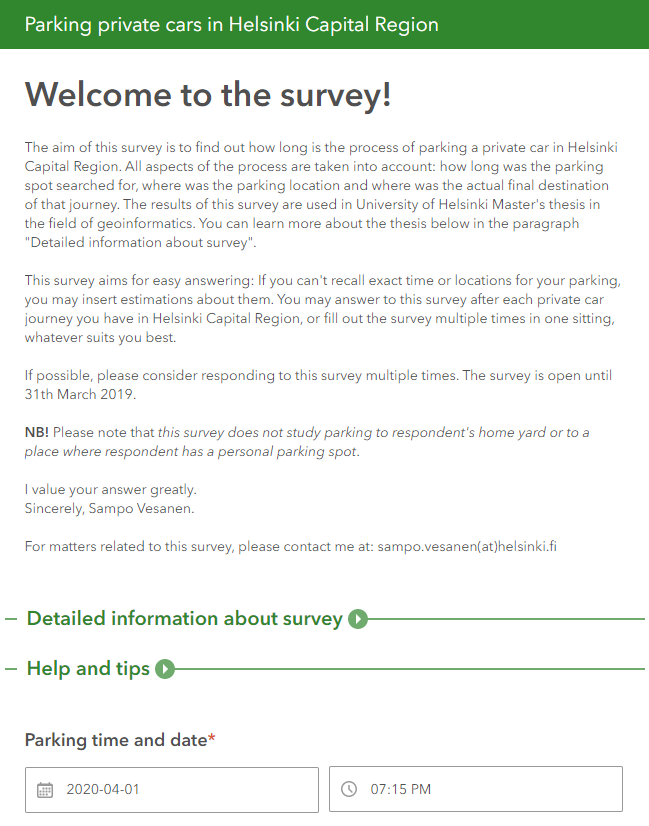
\includegraphics[width=5.5cm]{survey123_1.png} }}%
    \subfloat[label 2]{{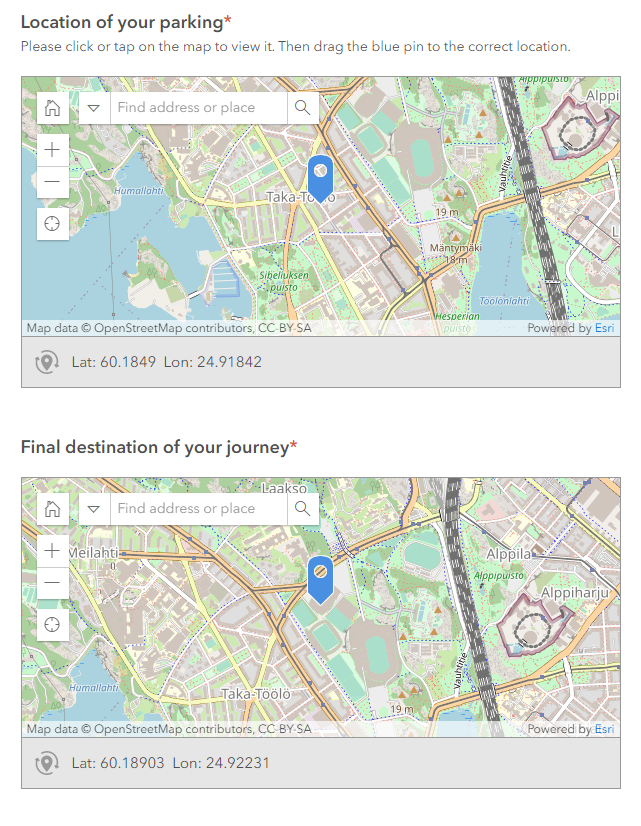
\includegraphics[width=5.5cm]{survey123_2.png} }}%
    \subfloat[label 3]{{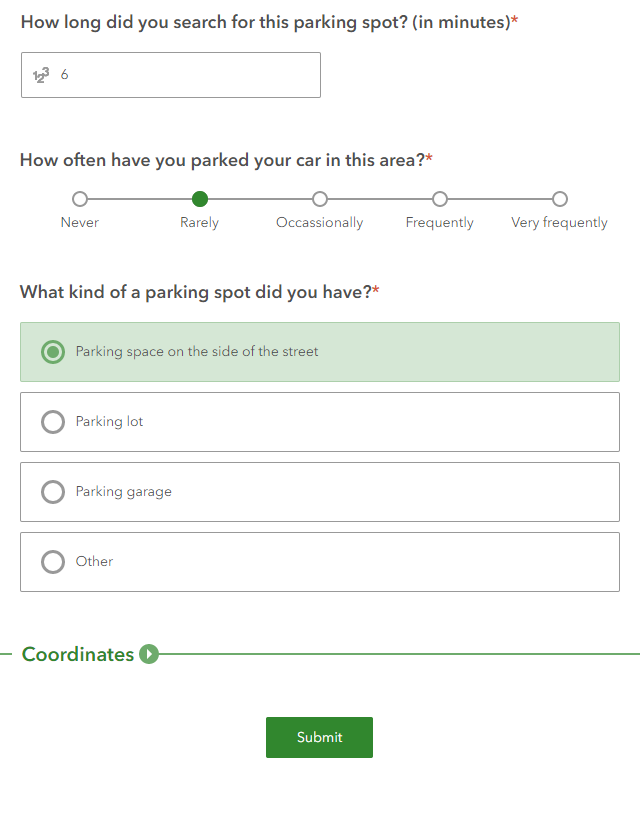
\includegraphics[width=5.5cm]{survey123_3.png} }}%
    \caption{Survey123 survey}%
    \label{fig:survey123}%
\end{figure}

In January 2019 the parking survey developed with Survey123 was deployed to friends and family, with a larger scale marketing push on social media platforms planned for later. At its core, this survey asked respondents for specific parking events in Helsinki Capital Region they had had. Respondents would pick an exact location on a map view for the location of their parked car and separately on a second map view the location of their final destination. Respondents were asked to do this for as many times as they had the will. The survey was released even after the Survey123 software had proved itself unwieldly for the purposes of this research. The software was difficult to use because of an arrangement of inconvenient design choices, unfinished functionality and multitude of bugs. It was not possible, for example, to have respondents leave multiple results at once. They would have to reload the survey, something a majority of people would not do. The desktop application of Survey123, Survey123 Connect, did not allow customisation of the post-submission message and therefore it would not be possible to efficiently direct respondents back to the form. Following the responses received by this form it was decided that the required spatial resolution for this research would need to be lower than exact points. Postal code areas were deemed an acceptable compromise in spatial accuracy. Specifying postal code areas as polygons in Survey123 was not possible. 

After careful consideration it was decided that the survey would have to be programmed from the ground up.

\subsubsection{Parking survey}
\justify
To achieve maximum transparency and repeatability for this research, a survey web application was programmed from the ground up. The survey and its supporting infrastructure was installed on a virtual machine in CSC's -- the state owned ICT solutions company -- Taito supercluster. Running on the Linux distribution Ubuntu version 16.04, the backbone of the survey ecosystem was a LAMP stack, a software bundle which incorporates the Linux operating system, Apache HTTP Server (web server software), \gls{mysql} relational database management system and the PHP programming language environment for server-side scripting. The visible component of the survey is the front-end, the only component of the survey system an user would interact with.

The front-end was programmed in NetBeans IDE 8.2.0 in JavaScript using an open-source mapping library Leaflet (software version 1.4.0) in January--May 2019. The survey was made available in English and Finnish languages. In the survey the respondent was presented with a map view of Helsinki Capital Region with its 167 postal code areas and was asked to fill out five questions about each area. User was asked to fill out as many postal code areas as they can remember parking in in last two years. Last two years was chosen as the timeframe to allow the respondent to comfortably think back while also forbidding the submission of out of date parking times. All answers received were estimates as the survey was not about an exact time and place. The answers were also subject to errors made by the user even though help functionality and a search tool were implemented in the parking survey. Once the user was finished with the survey, they would send them to the server. The user could return to the survey to add data on any postal code areas they had missed the last time. The survey questions are available for viewing in the appendices.

When data was received from the user, a \gls{php} language script verified the contents. This was an effort to prevent attacks on the web server running the study survey, as it was visible to the entire internet. Additionally, the verification made sure falsified or incomplete data would not find its way to the database containing the accepted results. Only specified variables were accepted from the survey. All of the variables had to be present in the received data, no unfinished results were accepted. As a failsafe if the verification test failed on any of the variables, user was informed about it. In addition to the verification, a PHP script tracked the IP addresses which had accessed the survey. By using the survey, respondents agreed that their IP addresses were recorded for the use of this thesis solely to recognise falsified or overlapping answers and detect unique visits. All IP addresses were anonymised with a Python script and original sensitive data deleted.

As a final survey component the server side contained two MySQL datatables, one for received records (Table~\ref{tab:recordstab}) and another for survey page hits (Table~\ref{tab:visitortab}). In the table \textit{records}, the following data was gathered: time of sending (timestamp), IP address (ip), postal code (zipcode), a value in the sequence 1--5 for the likert question (likert), a value in the sequence 1--4 for the question what type of parking spot was used (parkspot), an integer value for how long it usually took to park in this location (parktime), an integer value for how long it usually took to walk from parking place to one's destination (walktime) and a value in the sequence 1--4 for the question at what time of the day one usually parks in the location (timeofday). In the table \textit{records} it is notable that in the case an user sends the server data for multiple postal code areas each of the postal code areas take up their own row in the data table. Consequently, it was theoretically possible for one user to simultaneously submit 167 rows of data.

In the table \textit{visitors} the following data was gathered: IP address (ip), the timestamp of the first visit (ts\_first), the timestamp of latest visit (ts\_latest), the count of visits (count). In this table an IP address is only stored once. On the first visit of an IP address the row for that IP address is created in the data table with ts\_first and ts\_latest being identical. On further visits of that IP address the original row is appended with updated information in the columns ts\_latest and count.

The parking survey was released to the public in May 2019 and the active phase of gathering results continued until 30th June 2019. However, the survey remained open after the active period, receiving the last response in October 2019. The majority of the respondents were found through Facebook. Invitations to participate in the survey were sent to 112 city district and neighborhood groups with a theoretical reach of tens of thousands of people. Of the 112 posts, 63 were Helsinki centric groups, while Espoo had 22, Vantaa 15 and bordering municipalities 12. In addition to these groups invitation to participate were sent to two other Facebook groups, "Lisää kaupunki Helsinkiin" and the GIS profession group "GIS-velhot". It is not possible to conclusively differentiate from which group or city survey responses originated from. A clue about the survey's popularity in each city, however, may be gained from the table \textit{visitors} as posts to the groups were sent over multiple days. In addition to Facebook, an effort was also made to get faculty members and students of University of Helsinki to participate in the survey. A small amount of answers were collected with a tweet sent from the Twitter account of Digital Geography Lab. After initial invitation to participate, reminders were sent to the largest Facebook groups one month after the original post.

The source code for the survey described in this chapter and step-by-step information to set up an identical system is available at GitHub (\textcolor{blue}{\url{https://github.com/sampoves/parking-in-helsinki-region}}). As a side product, a variant of this survey was created where users pick precise points instead of areas. This precise survey template is, too, available at GitHub (\textcolor{blue}{\url{https://github.com/sampoves/leaflet-map-survey-point}}).

% \scalebox to prevent table going too wide
\begin{hyphenrules}{nohyphenation}
    \begin{table}[H]
        \centering
        \setlength\tabcolsep{1pt}
        \caption{Records} 
        \label{tab:recordstab}
        \scalebox{0.92}{\begin{tabular}{ @{} >{\raggedright\arraybackslash}p{1.5cm} >{\raggedright\arraybackslash}p{4cm} >{\raggedright\arraybackslash}p{2.5cm} >{\raggedright\arraybackslash}p{2cm} >{\raggedright\arraybackslash}p{1.5cm} >{\raggedright\arraybackslash}p{1.5cm} >{\raggedright\arraybackslash}p{1.5cm} >{\raggedright\arraybackslash}p{1.5cm} >{\raggedleft\arraybackslash}p{1.5cm} @{} }
            \toprule
            \cmidrule(r){1-2}
            id & timestamp & ip & zipcode & likert & parkspot & parktime & walktime & timeofday \\
            \midrule
            3244 & 2019-06-06 21:39:50 & wro4qo8hv4 & 00510 & 1 & 4 & 0 & 3 & 1 \\
            3245 & 2019-06-06 21:41:21 & aonm72lyx3 & 00520 & 2 & 1 & 10 & 5 & 1 \\
            3246 & 2019-06-06 21:41:54 & n1982i4i2v & 00100 & 1 & 1 & 20 & 4 & 1 \\
            3247 & 2019-06-06 21:46:19 & sbhfz0uvsl & 00210 & 1 & 1 & 5 & 3 & 3 \\
            3248 & 2019-06-06 21:46:22 & sbhfz0uvsl & 00220 & 2 & 2 & 5 & 5 & 2 \\        
            \bottomrule
        \end{tabular}}
    \end{table} 
\end{hyphenrules}

\begin{hyphenrules}{nohyphenation}
    \begin{table}[H]
        \centering
        \setlength\tabcolsep{1pt}
        \caption{Visitors} 
        \label{tab:visitortab}
        \begin{tabular}{ @{} >{\raggedright\arraybackslash}p{2cm} >{\raggedright\arraybackslash}p{3cm} >{\raggedright\arraybackslash}p{4cm} >{\raggedright\arraybackslash}p{4cm} >{\raggedleft\arraybackslash}p{1cm} @{} }
            \toprule
            \cmidrule(r){1-2}
            id & ip & ts\_first & ts\_latest & count \\
            \midrule
            1780 & mvovd467a7 & 2019-05-26 15:25:23 & 2019-05-26 15:26:06 & 2 \\
            1781 & xgbgkkzxb3 & 2019-05-26 15:26:23 & 2019-05-26 15:26:23 & 1 \\
            1782 & c9qer4q99a & 2019-05-26 15:27:25 & 2019-05-26 15:27:25 & 1 \\
            1783 & cujhd0hng7 & 2019-05-26 15:27:29 & 2019-05-26 15:27:29 & 1 \\
            1784 & 3ja7gjtko6 & 2019-05-26 15:28:45 & 2019-05-26 15:29:20 & 2 \\        
            \bottomrule
        \end{tabular}
    \end{table} 
\end{hyphenrules}

\subsection{Processing survey data}
\label{sec:processdata} % labeling to enable hyperref to this chapter
\justify
%% pidä postal df mukana, muuten on sekavaa

%\begin{itemize}
%    \item anonymisation of ip addresses
%    \item Read in spatial data sources
%    \item Read in survey data
%    \item Prepare source data (convert formats, remove some irregular erroneous answers from dataset)
%    \item Prepare shape files (remove islands not reachable by car)
%    \item give grid cells zipcodes (ykr grid does not have those of-the-shelf. Develop method to assign all cells zipcodes, take into account water and grid cells which are outside of research area)
%    \item respondent behaviour (see how each user has answered)
%    \item detect illegal data (first detect duplicate answers, produce report. Then remove data where parktime and/or walktime is 60 or over)
%    \item Add data to geodataframes (add columns for ykr\_vyoh, ua-forest, answer count, parktime and walktime mean
%    \item show statistics to user
%    \item Set percentage of urban zones and forest in each zipcode area (choose one urban zone and forest amount (jenks breaks) for every zipcode)
%    \item add subdivisions to data (all answer row gets corresponding subdivision value)
%    \item EXPERIMENTAL utilise travel-time matrix 2018, make comparisons
%    \item EXPERIMENTAL somehow create my own TTM18, with updated values
%    \item export results to R
%\end{itemize}

At the beginning of processing the research survey data, all IP addresses were anonymised. The anonymisation was carried out in such a way that the random identifiers for respondents matched in records and visitors, preserving the possibility to associate responses with survey visits. All data processing was carried out in Python 3.7.6, using Anaconda, a free and open-source Python distribution for scientific programming. Anaconda version 2020.02 included all essential packages for carrying out the script, except for the geospatial data package GeoPandas 0.5.0. GeoPandas and its dependencies -- GDAL 2.4.1, Fiona 1.8.6, pyproj 2.1.3, rtree 0.8.3, and Shapely 1.6.4.post1 -- were manually installed through Python package installer pip.

The main objective of data processing was to merge the survey results with spatial data. Using a selection of open data layers, new explanatory spatial data would be available for analysis (see table \ref{tab:useddata}). This opened opportunities to compare the new survey data against that currently present in Helsinki Travel-time Matrix 2018.

The data processing started with loading aforementioned open spatial data and selecting only those areas relevant to the research. Postal code areas were processed to only include areas reachable by car from the mainland in the research area. Islands not reachable by car were approximated visually using Google Maps.

Helsinki Travel-time Matrix 2018 and the survey data of this thesis operate in different spatial units. Travel-time Matrix 2018 uses the 250 x 250 meter Statistics Finland statistics grid and the basic spatial unit of the survey data is the zip code area. Using Python, postal codes were added to each grid cell with the logic that the largest area (\textcolor{red}{LISÄÄ KUVA}) assigns the postal code. PAAVO postal code areas are not present in all of the cells of YKR statistics grid and because of this some cells have a postal code of 99999 to denote missing data. In addition, the grid was merged with data which tells how much of a cell is contained in the research area and how large is the largest share which dictated the denotation of the current cell.

The data processing script created for this thesis contains detailed features to detect patterns in the survey data. To enable pattern recognition the records were purged of known false data, namely records and visits made by the author. In addition, one survey user reported that they had inserted erroneous data in the survey. These responses were identified and deleted.

A Pandas DataFrame was created to make it easy to view the behaviour of each survey respondent. In addition to this feature, the data processing script writes a text file format report about respondents who have submitted multiple responses from the same postal code area. This report was then used to determine what to do about the duplicates.

It was decided that if parking time or walking time value was over 60 minutes that value would be deleted. This value is arbitrary and there is little reason (\textcolor{red}{voiko sanoa näin, hatusta heitetty?}) to believe that it would take anyone 60 minutes to reach their final destination from their place of parking. An hour of searching for parking plausible in the center of Helsinki. The data processing script deleted, additionally, the illegal IP address codes from visitors.

Next the additional spatial data was added to the survey data. Postal dataframe was added with answer count, parking time mean and walking time mean. Each postal code area also received seven columns to depict the share of classes in percentage. Using Urban Atlas 2012 data, all postal code areas were tested for forest percentage. Using a custom Jenks breaks function (by GitHub user Drewda, \textcolor{red}{miten citation?}) suitable class breaks were calculated to be used in records.

The dataframe records would be used as data in the analysis part of the thesis. Using the calculations made for dataframe postal, each row in records would receive, according to their postal code area, the most common urban structure type and the most common jenks break value. With data gathered from the Helsinki Capital Region web sites, using the postal code area in each response, the city subdivisions (Finnish "suuralue") were added to the dataframe records.

The source code for the data processing described in this chapter is available at GitHub (\textcolor{blue}{\url{https://github.com/sampoves/Msc-thesis-data-analysis}}).

\subsection{Conducting analyses}
% - Compare a few different travel time chains in Helsinki Capital Region. A few starting points and a few finishing points
% - All of the statistics stuff to detect the variation 
% - Tuuli was supposed to send me the exact numbers used for parking in Travel Time Matrix, did not do it yet

%\begin{itemize}
%    \item Prepare data to R compliant format
%    \item ShinyApp descriptive statistics
%    \item shinyapp histogram for parktime and walktime
%    \item shinyapp boxplot, show outliers
%    \item shinyapp barplot, show amounts
%    \item shinyapp levene test
%    \item shinyapp one-way anova
%    \item shinyapp map, nice to have, not at all important
%    \item visitor shinyapp, see the accumulation of visits and received records
%\end{itemize}
\justify
Once data processing in Python was completed, the survey data was carried over to R for its easy to access statistical analysis functionality (namely packages \textit{onewaytests} for ANOVA and Brown-Forsythe test, \textit{plotrix} for standard error, and \textit{moments} for quantiles) \textcolor{red}{citation}. To help viewing the large dataset of survey results, two Shiny applications were written, one for records and a second for visitors. The significance of this decision was twofold. Firstly, the interactive application allows switching variables on and off in the statistical tests in real time, making survey results analysis more efficient. Secondly, Shiny applications can be deployed to the Internet using the website shinyapps.io. This makes it effortless to display the results of this thesis in a visual way and uphold the thesis' mission of transparency as everyone can inspect the results and the tool themselves.

In the records tool users can view the survey data from multiple different angles. Users are given control which variables are active at any moment. The basis for the tool are the dropdown menus for continuous variables parktime and walktime and ordinal variables likert, parkspot, timeofday, ua\_forest, ykr\_zone, and subdiv. Any and all groups of values in the ordinal variables can be deactivated to better understand significance of each value. In addition to the selection of the continuous and ordinal variable, users can deactivate records based on their spatial location in research area subdivisions.

When the user has selected a continuous and an ordinal variable to compare, they are presented a thorough set of descriptive statistics with n, median, mean, standard deviation, standard error, confidence interval for lower and upper bound, minimum and maximum, 25 \% and 75 \% quantiles, skewness and kurtosis. For the continuous variables, a histogram is available to visualise the distribution of walktime and parktime. Distribution of ordinal variables likert, parkspot and timeofday can be compared against other ordinal variables in a barplot. To study quartiles, a boxplot is available. Imprortantly, users can test their selection of variables using the test of homogeneity of variables (Levene's test), analysis of variance (ANOVA), and the Brown-Forsythe test. Lastly, a context map of the research area is provided. The purpose of this map is to visualise which subdivisions are currently selected and which are deactivated.

Users can deactivate specific values from the currently selected ordinal variable at any time. In addition to this subdivisions of research area cities can be deactivated flexibly to better understand the spatial differences of the cities.

In visitors research tool users can view and examine events in the timeline of the survey research. In an interactive view cumulative charts are presented for received responses and survey page first visits. The charts reveal the effect of advertisement on actual records and survey traffic. Significance of different sources of responses can be viewed.

Scripts described in this chapter were written in RStudio 1.2.5033 using R for Windows 3.6.3. The source code for the data analysis and visualisation scripts are available at GitHub (\textcolor{blue}{\url{https://github.com/sampoves/Msc_thesis_data_analysis}}). The interactive analysis tools are available for testing on Shinyapps.io (\textcolor{blue}{\url{https://sampoves.shinyapps.io/records}} and  \textcolor{blue}{\url{https://sampoves.shinyapps.io/visitors}}). 